\documentclass[conference]{IEEEtran}

% ── Packages ──────────────────────────────────────────────────────────────────
\usepackage[T1]{fontenc}
\usepackage[utf8]{inputenc}
\usepackage{cite}
\usepackage{amsmath,amssymb}
\usepackage{graphicx}
\usepackage{booktabs}
\usepackage{array}
\usepackage{tabularx}
\usepackage{multirow}
\usepackage{url}
\usepackage[colorlinks=true,urlcolor=blue,linkcolor=black,citecolor=black]{hyperref}
\usepackage{xcolor}
\usepackage{listings}

\lstset{
  basicstyle=\ttfamily\footnotesize,
  breaklines=true,
  frame=single,
  backgroundcolor=\color{gray!8}
}

% ─────────────────────────────────────────────────────────────────────────────
\begin{document}

\title{AgroSense: Satellite-Based Crop Stress Classification and Smart Farming
       Decision Support for Pakistan Smallholder Agriculture}

\author{
  \IEEEauthorblockN{Ali Shahmeer \quad Basit Hassan, MS \quad Kabir Ghoto, PhD}
  \IEEEauthorblockA{
    \textit{Department of Software Engineering}\\
    \textit{Sindh Madressatul Islam University}\\
    Karachi, Pakistan\\
    areo5459@gmail.com
  }
}

\maketitle

% ── Abstract ──────────────────────────────────────────────────────────────────
\begin{abstract}
Pakistan's agricultural sector, contributing approximately 24\% of GDP while
employing over 37\% of the national workforce, continues to incur significant
crop losses attributable to water stress, disease outbreaks, and sub-optimal
input application. Conventional field scouting is labour-intensive, infrequent,
and dependent on expert availability. This paper presents AgroSense, an
integrated agricultural intelligence platform that processes Sentinel-2
satellite imagery via Google Earth Engine (GEE), runs five machine learning
models, and delivers real-time weather intelligence from Open-Meteo. The system
provides crop-condition monitoring, irrigation recommendations, yield
forecasting, soil health assessment, and variable-rate application (VRA) zone
mapping through a cross-platform Flutter mobile application, a bilingual
(English/Urdu) desktop application, and a RESTful API deployed on Google Cloud
Run. For the crop-condition proxy classification task, a comparative evaluation
of five ML algorithms---Random Forest, XGBoost, Gradient Boosting, SVM~(RBF),
and $k$-NN---is conducted on 1,786 Sentinel-2 observations from 99
georeferenced agricultural sampling locations (district/city-centroid buffers)
across all four provinces (Punjab, Sindh, Balochistan, and KPK), spanning 19
crop-season windows from 2015 to 2024, collected via the GEE API. Class labels
(Healthy / Stressed / Diseased) are spectrally derived proxy classes generated
from a vegetation health composite; the input features NDVI, NDRE, and EVI also
participate in label generation. Evaluation uses a location-grouped train/test
split (\texttt{GroupShuffleSplit} on sampling-location identifiers) and nested
5-fold \texttt{StratifiedGroupKFold} cross-validation with \texttt{GridSearchCV}
hyperparameter tuning. SVM~(RBF) achieves the highest held-out test accuracy
(98.34\%) and XGBoost achieves the best nested cross-validated macro F1 (0.983).
Random Forest (96.40\% test accuracy, nested CV macro F1~=~0.980) is selected
as the production model for interpretability. Reported results represent an
upper bound on spectral proxy separability rather than independently validated
crop disease detection.
\end{abstract}

\begin{IEEEkeywords}
Crop stress classification, Google Earth Engine, machine learning, NDVI,
Pakistan, precision agriculture, Random Forest, satellite remote sensing,
Sentinel-2, smart farming.
\end{IEEEkeywords}

% ─────────────────────────────────────────────────────────────────────────────
\section{Introduction}

Pakistan's agricultural sector, which contributes approximately 24\% of GDP and
employs over 37\% of the national workforce~\cite{pbs2024,pesurvey2025}, faces
persistent crop losses attributable to preventable causes---water stress,
disease, and sub-optimal fertiliser application---that remain elevated despite
decades of government intervention. Smallholder farms, which
constitute the majority of cultivated area across Punjab and Sindh, lack access
to timely, actionable crop health intelligence. The Indus basin irrigation
system, which supports an estimated 17 million hectares of irrigated cropland,
faces compounding pressures from water scarcity and secondary
salinisation~\cite{muzammil2020}. Satellite remote sensing combined with machine
learning offers a scalable alternative: field conditions can be assessed at
10-metre spatial resolution on a 5-day revisit cycle using the Sentinel-2
constellation~\cite{drusch2012} without requiring physical site visits.

Vegetation indices computed from multispectral imagery---particularly NDVI,
EVI, and NDRE---have been shown to correlate strongly with crop health,
chlorophyll content, and water stress~\cite{rouse1974,gitelson2002}. Emerging
remote sensing platforms and cloud-based geospatial APIs have substantially
lowered the computational barrier to field-scale crop monitoring in
under-resourced agricultural research contexts~\cite{sishodia2020}. Google
Earth Engine (GEE)~\cite{gorelick2017} enables cloud-scale processing of
petabytes of satellite imagery, removing infrastructure barriers that previously
confined such pipelines to well-resourced institutions. Ensemble classifiers
such as Random Forest~\cite{breiman2001} and gradient boosting
variants~\cite{chen2016xgboost} have demonstrated competitive performance on
small-to-medium agricultural datasets, making them well-suited for deployment
contexts where large labelled datasets are expensive to acquire.

AgroSense addresses the disconnect between satellite-derived insights and
actionable farm management by providing an end-to-end pipeline from raw
satellite imagery to mobile-accessible recommendations. The system targets five
critical decision points in crop management: (1)~crop health monitoring through
early stress and disease detection; (2)~irrigation management for optimal timing
and volume; (3)~yield forecasting for harvest readiness estimation; (4)~soil
health assessment of pH, salinity, and organic matter; and (5)~variable-rate
application (VRA) zone mapping for precision fertiliser scheduling.

The principal contributions of this paper are:
\begin{enumerate}
  \item An end-to-end satellite-to-recommendation pipeline integrating GEE,
        five specialised ML models, and real-time weather intelligence within a
        single cloud-native platform serving both mobile and desktop clients.
  \item A comparative evaluation of five classification algorithms on
        Sentinel-2 spectral indices for spectral proxy crop-condition
        classification under Pakistan agronomic conditions, using location-grouped
        evaluation with nested cross-validation. Labels are derived from the same
        spectral indices used as features (see Section~\ref{sec:experiments});
        results quantify proxy-class separability, not independently validated
        crop-disease diagnosis.
  \item A bilingual (English/Urdu) cross-platform interface design enabling
        farmer and agronomist accessibility across Pakistan's linguistic
        landscape.
  \item A crop-condition proxy dataset comprising 1,786 Sentinel-2 Level-2A
        observations collected via Google Earth Engine from 99 georeferenced
        agricultural sampling locations (district/city-centroid buffers) across
        all four provinces of Pakistan, spanning 19 crop-season windows from
        2015 to 2024, released as a reproducible evaluation benchmark at
        \url{https://github.com/ALI-SHAHMEER/agrosense-pakistan-crop-stress}.
        Labels are spectrally derived proxy classes; independent agronomic
        ground-truth validation is future work.
\end{enumerate}

% ─────────────────────────────────────────────────────────────────────────────
\section{Related Work}

\subsection{Remote Sensing for Crop Monitoring}

Satellite-based crop monitoring has been extensively validated across diverse
agricultural systems. Rouse \textit{et al.}~\cite{rouse1974} established NDVI
as a quantitative proxy for vegetation vigour, while Gitelson \textit{et
al.}~\cite{gitelson2002} demonstrated that EVI and red-edge-based indices offer
chlorophyll-sensitive characterisation superior to broadband NDVI in dense
canopies. The Sentinel-2 constellation, with its 10~m spatial resolution and
5-day revisit cycle, has since become the preferred source for plot-scale crop
monitoring~\cite{immitzer2016}. Tamiminia \textit{et al.}~\cite{tamiminia2020},
in a meta-analysis of 349 peer-reviewed GEE-based studies, confirmed that
optical satellite imagery processed with Random Forest constitutes the most
widely adopted paradigm for agricultural land monitoring at regional and global
scales. Htitiou \textit{et al.}~\cite{htitiou2020} demonstrated that
phenological metrics derived from Sentinel-2 NDVI and EVI time series
substantially improve crop type discrimination over single-date classification,
achieving 88\% overall accuracy with Random Forest. Omia \textit{et
al.}~\cite{omia2023} provide a comprehensive review of spectral imaging
technologies for field crop monitoring, confirming that this satellite--ML
combination remains the leading methodology for scalable crop health assessment.
Ojeilua \textit{et al.}~\cite{ojeilua2025} reviewed satellite and drone-based
stress detection in developing-region agricultural systems, identifying NDVI,
NDWI, and red-edge reflectance as the most diagnostically informative spectral
features for drought, salinity, and nutrient stress. Most published systems
process imagery in scheduled batch mode~\cite{tamiminia2020,htitiou2020};
AgroSense instead provides on-demand analysis triggered directly from a mobile
interface.

\subsection{Machine Learning in Precision Agriculture}

Karthikeyan \textit{et al.}~\cite{karthikeyan2020} survey ML methods in
precision agriculture and identify ensemble classifiers---particularly Random
Forest---as the dominant approach for crop health classification on field-scale
datasets, owing to their robustness under small sample sizes and mixed feature
types. XGBoost~\cite{chen2016xgboost} has demonstrated competitive or superior
results on tabular agricultural data, while kernel-based SVMs have demonstrated
strong performance on high-dimensional hyperspectral classification tasks.
Maleki \textit{et al.}~\cite{maleki2024} demonstrated that combining
Sentinel-1 SAR backscatter with Sentinel-2 vegetation indices achieves mean F1
scores of 89.9--93.5\% for summer crop mapping, with XGBoost outperforming
Random Forest and Multi-Layer Perceptron in multi-sensor configurations. Our
comparative study directly evaluates these methods on Pakistan Sentinel-2 data,
contributing benchmark results absent from prior literature for this geographic
and agronomic context.

\subsection{Smart Farming Decision Support Systems}

Several platforms integrate satellite indices with weather data for farm
management support. Wolfert \textit{et al.}~\cite{wolfert2017} characterise the
``Big Data in Smart Farming'' paradigm, emphasising the need for systems that
establish a feedback cycle from field sensing to farm management decision.
Leading commercial precision agriculture platforms provide comparable
functionality but target large-scale mechanised farms in North America and
Europe. AgroSense is specifically designed for smallholder farms in South Asia,
with explicit Urdu localisation and a zero-cost weather data source
(Open-Meteo~\cite{zippenfenig2023}).

\subsection{Yield Prediction and Crop Health in Pakistan}

Remote sensing-based yield estimation has been validated at regional and field
scales across diverse agronomic contexts. Ashfaq \textit{et
al.}~\cite{ashfaq2025} introduced DeepAgroNet, a three-branch deep learning
framework integrating GEE-processed satellite imagery, meteorological data, and
soil characteristics for winter wheat yield prediction at the district level in
southern Pakistan, with the CNN branch achieving an $R^2$ of 0.77 one month
prior to harvest. Jamil \textit{et al.}~\cite{jamil2025} demonstrated that
Sentinel-derived vegetation indices---including NDVI, EVI, SAVI, GDVI, and
IVI---exhibit strong polynomial relationships with wheat crop age and health in
Punjab, Pakistan, reporting $R^2$ values of 0.68--0.92. AgroSense's yield
predictor integrates growing-degree features with temporal NDVI statistics and
is calibrated against Pakistan Bureau of Statistics 2024 provincial
averages~\cite{pbs2024} for wheat, rice, cotton, sugarcane, and mango---crops
that collectively represent the majority of Pakistan's cultivated area.

Collectively, the reviewed literature confirms the technical feasibility of
satellite-based crop monitoring but reveals a consistent gap: no existing open
system integrates GEE-derived spectral analysis, multi-model ML inference, and
real-time weather intelligence within a single mobile-accessible platform
calibrated for Pakistan's smallholder context. AgroSense directly addresses
this gap.

% ─────────────────────────────────────────────────────────────────────────────
\section{System Architecture}

The system follows a three-tier architecture illustrated in
Fig.~\ref{fig:architecture}. This separation was chosen to decouple
computationally intensive satellite processing and ML inference from the client
tier, enabling a single stateless API to serve both mobile and desktop
interfaces without duplicating business logic. A satellite ingestion layer
fetches and preprocesses Sentinel-2 and Landsat-8 imagery via GEE. A FastAPI
backend~\cite{fastapi} running on Google Cloud Run performs ML inference and
exposes a RESTful API. Two client tiers---a Flutter mobile
application~\cite{flutter} and a PyQt6 desktop application---consume the API
independently.

\begin{figure}[htbp]
  \centering
  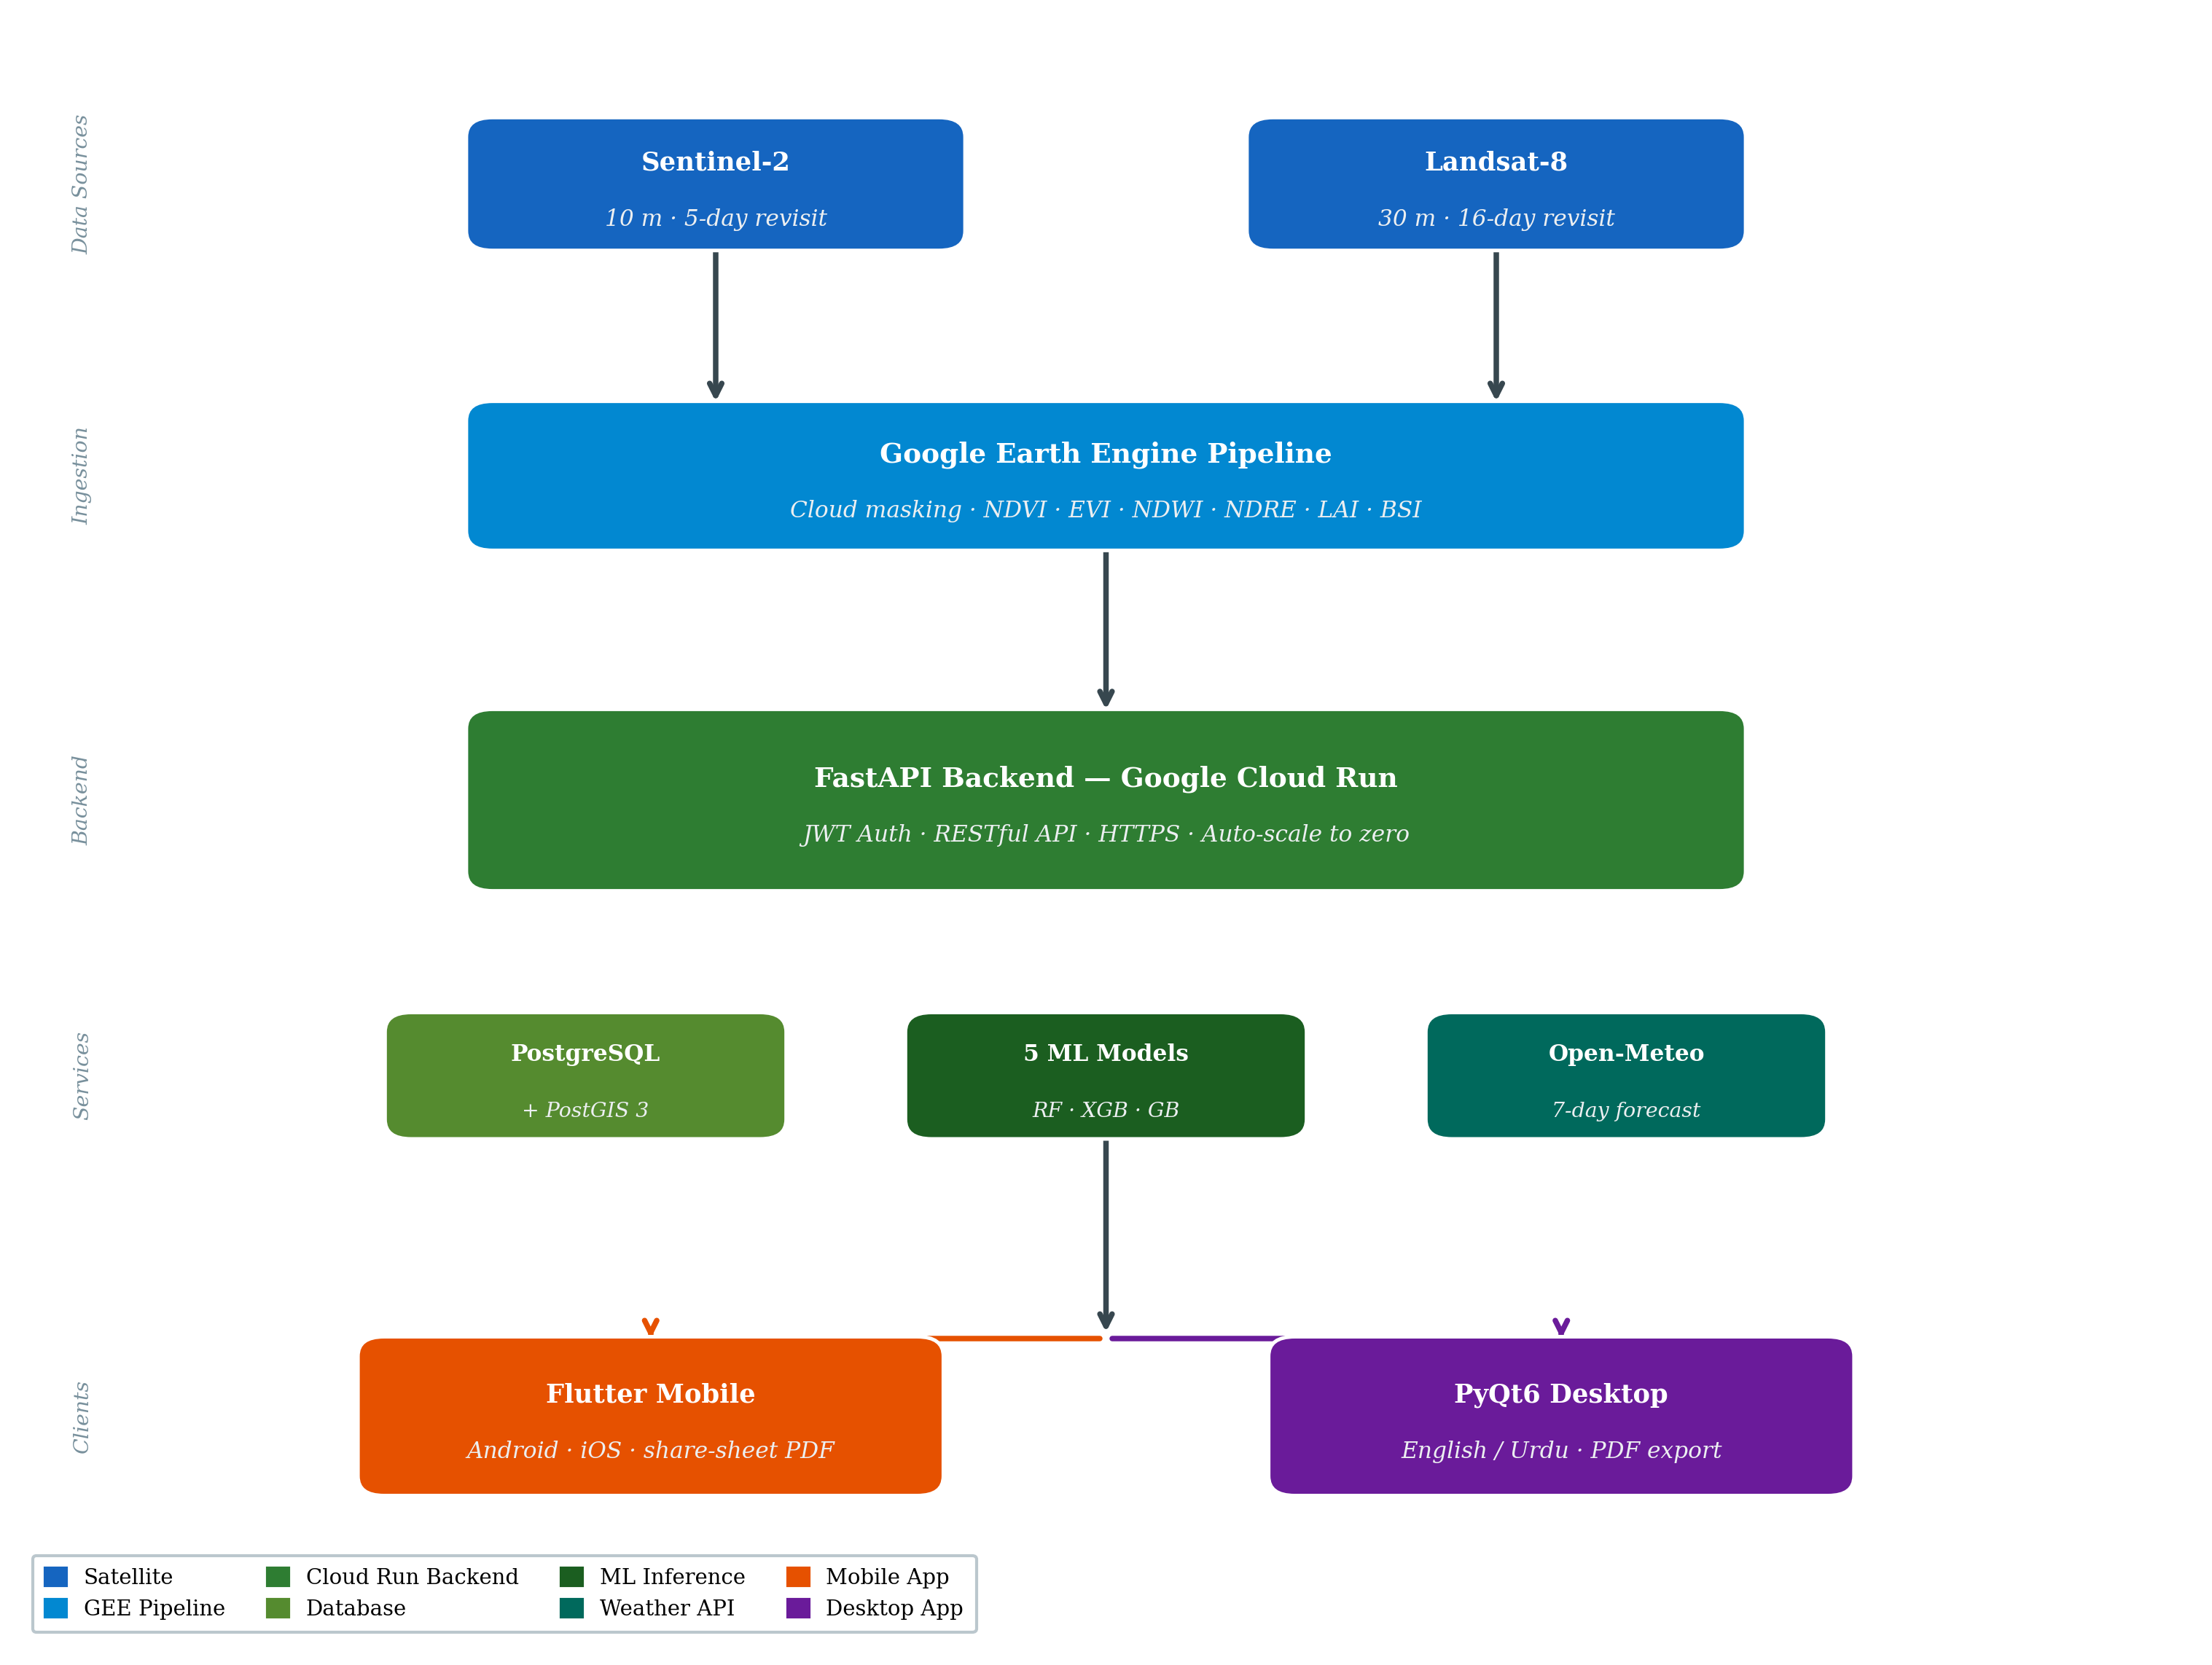
\includegraphics[width=\columnwidth]{fig1_architecture.png}
  \caption{AgroSense three-tier system architecture.}
  \label{fig:architecture}
\end{figure}

\subsection{Backend Technology Stack}

Technology selection prioritised open-source components with strong geospatial
and ML ecosystems and zero per-request licensing cost.
Table~\ref{tab:stack} summarises the key backend components.

\begin{table}[htbp]
  \caption{Backend Technology Stack}
  \label{tab:stack}
  \centering
  \begin{tabular}{ll}
    \toprule
    \textbf{Component} & \textbf{Technology} \\
    \midrule
    API Framework      & FastAPI 0.111~\cite{fastapi}, Uvicorn \\
    Database           & PostgreSQL 16 + PostGIS 3~\cite{postgis} \\
    ORM / Migrations   & SQLAlchemy 2.0, Alembic \\
    Satellite Pipeline & GEE API (earthengine-api 0.1.403)~\cite{gorelick2017} \\
    ML Runtime         & scikit-learn 1.4.2~\cite{sklearn}, XGBoost 2.0.3~\cite{chen2016xgboost} \\
    Geospatial         & Rasterio 1.3.10, Shapely 2.0.4 \\
    Weather            & Open-Meteo~\cite{zippenfenig2023} \\
    Authentication     & JWT (python-jose), bcrypt \\
    PDF Generation     & ReportLab 4.2.5~\cite{reportlab}, arabic-reshaper \\
    Deployment         & Docker, Google Cloud Run \\
    \bottomrule
  \end{tabular}
\end{table}

\subsection{Mobile Application}

The mobile application is built with Flutter 3.44~\cite{flutter} (Dart~3.12),
targeting Android (API~21+) and iOS from a single codebase. The application
constitutes the primary interface through which farmers and agronomists interact
with the AgroSense platform.

\subsubsection{Architecture and State Management}
The application follows a reactive widget architecture with a language switcher
backed by observable state. All API communication is encapsulated in a singleton
service layer that attaches a JWT Bearer token to every request; tokens are
persisted locally across sessions. As a security design principle, no
third-party credentials---GEE, Open-Meteo, or Gmail SMTP---are embedded in the
client binary; all such secrets are held exclusively server-side on Cloud Run.

\subsubsection{Screen Structure}
Navigation is managed by a \texttt{MainShell} scaffold with a persistent
field selector. The application comprises eight screens:

\begin{itemize}
  \item \textbf{LoginScreen} --- JWT-based authentication with persistent
        token storage across sessions.
  \item \textbf{FarmsScreen} --- Farm and field management; field boundaries
        are defined by GPS polygon coordinates submitted to the PostGIS backend.
  \item \textbf{DashboardScreen} --- The core analysis screen. A single user
        interaction triggers a sequential four-stage pipeline: (1)~satellite
        fetch via GEE, (2)~five ML model inference, (3)~current weather fetch,
        and (4)~temporal NDVI anomaly detection. Results are displayed as
        colour-coded cards with severity badges, providing a complete crop
        health snapshot without requiring the user to navigate multiple screens.
  \item \textbf{AnalyticsScreen} --- Interactive time-series charts of NDVI
        and other spectral indices over a rolling 12-month window.
  \item \textbf{ImageryScreen} --- Satellite imagery viewer with multi-band
        selection (RGB true colour, NDVI false colour).
  \item \textbf{SmartFarmingScreen} --- Seven-day weather forecast cards,
        active alert list with severity indicators, and ideal planting date
        recommendation.
  \item \textbf{ProfileScreen} --- User account management.
\end{itemize}

\subsubsection{PDF Export}
The PDF export subsystem uses a platform-conditional import pattern
(\texttt{pdf\_saver\_mobile.dart} / \texttt{pdf\_saver\_web.dart} /
\texttt{pdf\_saver\_stub.dart}) to support both Android/iOS and potential
web targets. On mobile, the ReportLab~\cite{reportlab}-generated PDF is
streamed from the backend and shared via the system share sheet.

\subsection{Desktop Application}

The PyQt6 desktop application provides a bilingual (English/Urdu) interface
targeted at agronomists and extension workers. It includes satellite imagery
visualisation with multi-band selection (RGB, NDVI false-colour, band
arithmetic), time-series analytics with interactive charts, and
ReportLab~\cite{reportlab}-based PDF report generation with correct Urdu text
shaping. NotoNaskhArabic was selected over NotoNastaliqUrdu, as the latter requires
GSUB/GPOS OpenType shaping not supported by the ReportLab rendering engine.

% ─────────────────────────────────────────────────────────────────────────────
\section{Satellite Data Pipeline}

Field boundaries are stored as PostGIS~\cite{postgis} polygons defined by GPS
coordinates. On analysis trigger, the pipeline: (1)~authenticates with GEE
using a service account; (2)~queries Sentinel-2 SR imagery for the field
polygon over a rolling 12-month window; (3)~applies QA60 cloud masking; and
(4)~computes six spectral indices as defined in Table~\ref{tab:indices}.

\begin{table}[htbp]
  \caption{Spectral Indices Computed from Sentinel-2}
  \label{tab:indices}
  \centering
  \renewcommand{\arraystretch}{1.35}
  \begin{tabular}{p{0.85cm} p{3.9cm} p{2.4cm}}
    \toprule
    \textbf{Index} & \textbf{Formula} & \textbf{Interpretation} \\
    \midrule
    NDVI &
      $\dfrac{B_8 - B_4}{B_8 + B_4}$ &
      Vegetation vigour~\cite{rouse1974} \\[6pt]
    EVI &
      $2.5\cdot\dfrac{B_8 - B_4}{B_8 + 6B_4 - 7.5B_2 + 1}$ &
      Canopy-corrected vigour~\cite{gitelson2002} \\[6pt]
    NDWI &
      $\dfrac{B_3 - B_8}{B_3 + B_8}$ &
      Canopy water / irrigation stress~\cite{karthikeyan2020} \\[6pt]
    NDRE &
      $\dfrac{B_{8A} - B_5}{B_{8A} + B_5}$ &
      Chlorophyll / early stress~\cite{gitelson2002,clevers2013} \\[6pt]
    LAI &
      $3.618\,\mathrm{EVI} - 0.118$ &
      Leaf area index~\cite{xie2019} \\[4pt]
    BSI &
      $\dfrac{B_{11}+B_4-B_8-B_2}{B_{11}+B_4+B_8+B_2}$ &
      Bare soil exposure~\cite{omia2023} \\
    \bottomrule
  \end{tabular}
\end{table}

\subsection{Spectral Index Interpretation}

Each index exploits specific spectral properties of vegetation and soil:

\textbf{NDVI} (Normalized Difference Vegetation Index) exploits the contrast
between chlorophyll absorption in the red band ($B_4$, 665~nm) and strong NIR
reflectance of the mesophyll cell structure ($B_8$, 842~nm). Values range from
$-1$ to $+1$; healthy crops typically yield values of 0.6--0.9, stressed or
sparse vegetation 0.2--0.5, and bare soil below 0.2.

\textbf{EVI} (Enhanced Vegetation Index) extends NDVI by incorporating a blue
band ($B_2$, 490~nm) correction that attenuates aerosol scattering artefacts,
alongside a canopy background adjustment factor. EVI exhibits reduced saturation
in dense canopies where NDVI plateaus at LAI~$\approx$~3, rendering it more
sensitive for high-biomass crops such as sugarcane and rice.

\textbf{NDWI} (Normalized Difference Water Index) uses the contrast between
green ($B_3$, 560~nm) and NIR ($B_8$, 842~nm). This green-NIR formulation is
sensitive to open-water bodies and surface-water presence; it also responds to
canopy moisture conditions at the landscape scale. Negative values indicate
denser or drier vegetation; values approaching $+1$ indicate open water or
saturated surfaces. In AgroSense it is used as a surface/open-water-sensitive
spectral index. Note: a shortwave-infrared formulation using NIR/SWIR bands
would be more specific to vegetation liquid-water content in future iterations.

\textbf{NDRE} (Normalized Difference Red-Edge Index) exploits Sentinel-2's
red-edge band ($B_5$, 705~nm), which occupies the steep reflectance transition
between chlorophyll absorption and NIR reflection. Clevers and
Gitelson~\cite{clevers2013} established that red-edge bands on Sentinel-2
provide highly accurate estimates of canopy chlorophyll and nitrogen content,
outperforming conventional broad-band indices. Boiarskii and
Hasegawa~\cite{boiarskii2019} further demonstrated that NDRE detects
nitrogen-limited chlorophyll depletion more sensitively than NDVI under
early-stage stress conditions, as chlorophyll degradation shifts the red-edge
reflectance transition before a corresponding NDVI decline becomes detectable,
making NDRE a temporally leading indicator of crop stress within the pipeline.

\textbf{LAI} (Leaf Area Index) is derived algebraically from EVI as
$\mathrm{LAI} = 3.618\,\mathrm{EVI} - 0.118$~\cite{xie2019}. Xie
\textit{et al.}~\cite{xie2019} validated Sentinel-2 red-edge bands for
retrieving LAI from winter wheat, demonstrating RMSE of 1.53~m$^2$/m$^2$.
Values above 4 indicate dense, healthy canopy; values below 2 indicate sparse
or stressed vegetation.

\textbf{BSI} (Bare Soil Index) uses SWIR ($B_{11}$, 1610~nm) alongside visible
and NIR bands to isolate exposed soil signal. Elevated BSI values flag land with
minimal vegetative cover and are used to support soil health classification and
detect field degradation between crop cycles.

Computed indices are persisted to the PostgreSQL \texttt{VegetationIndex} table
and serve as input features for all five ML models. Incoming NDVI values are
also compared against a per-field seasonal baseline; deviations trigger temporal
anomaly alerts at Watch ($-10\%$), Warning ($-20\%$), and Critical ($-30\%$)
severity levels.

% ─────────────────────────────────────────────────────────────────────────────
\section{Machine Learning Models}

The crop-condition classifier is trained on 1,786 Sentinel-2 Level-2A
observations collected via the GEE API from 99 georeferenced agricultural
sampling locations (district/city-centroid buffers, ~1~km radius) across all
four provinces (Punjab, Sindh, Balochistan, and KPK), spanning 19 crop-season
windows from 2015 to 2024 (10 Kharif, 9 Rabi). Five crops are represented:
wheat (883, 49.4\%), rice (308, 17.2\%), cotton (272, 15.2\%), sugarcane
(216, 12.1\%), and mango (107, 6.0\%), derived programmatically from the
published CSV. The remaining four decision-support modules (irrigation,
yield, soil health, VRA zones) are prototype components calibrated against
Pakistan Bureau of Statistics 2024 provincial averages~\cite{pbs2024}
and pending task-specific validation datasets.

\subsection{Crop Stress Classification}

A Random Forest classifier~\cite{breiman2001} is trained on nine
Sentinel-2-derived spectral features: NDVI, EVI, NDWI, NDRE, LAI, BSI,
NDVI\_std, NDVI\_min, and NDVI\_max. The three output proxy classes are
\textit{Healthy}, \textit{Stressed}, and \textit{Diseased}. These labels
are derived from a vegetation health composite (0.5$\cdot$NDVI +
0.3$\cdot$NDRE + 0.2$\cdot$EVI) via tertile split; the same NDVI, NDRE, and
EVI are also input features, creating a known label-circularity relationship.
Reported performance measures spectral proxy separability and is an upper bound
relative to independently validated disease detection.

\subsection{Irrigation Recommendation}

An XGBoost classifier~\cite{chen2016xgboost} maps NDWI, NDVI, LAI,
estimated soil moisture (derived from NDWI), forecast temperature, and
precipitation to one of four recommendations: \textit{Irrigate Now},
\textit{Irrigate Soon}, \textit{Adequate}, or \textit{Overwatered}.

\subsection{Yield Prediction}

A Random Forest regressor~\cite{breiman2001} predicts yield in tonnes per
hectare from NDVI, NDVI\_max, EVI, NDRE, LAI, growing\_days, and weather
covariates (rainfall and temperature) sourced from
Open-Meteo~\cite{zippenfenig2023}, together with crop type. This approach is
consistent with satellite-based yield estimation frameworks validated for
Pakistani wheat agriculture by Ashfaq \textit{et al.}~\cite{ashfaq2025} and
Jamil \textit{et al.}~\cite{jamil2025}.
Pakistan Bureau of Statistics 2024 baselines~\cite{pbs2024} are used for
calibration: wheat 3.1, rice 4.1, cotton 1.6, sugarcane 58.0, and
mango 8.5~t/ha.

\subsection{Soil Health Assessment}

Three independent Gradient Boosting regressors predict soil pH, salinity
(dS/m), and organic matter percentage from NDVI, NDWI, BSI, and Sentinel-2
bands $B_2$, $B_3$, $B_4$, $B_8$, and $B_{11}$. Salinity prediction is
particularly critical for Indus basin fields where secondary salinisation
represents a persistent and spatially extensive agricultural challenge.

\subsection{Variable-Rate Application Zones}

A Random Forest classifier~\cite{breiman2001} maps NDVI, NDRE, NDWI, EVI,
LAI, and NDVI\_std to one of three fertiliser application zones:
\textit{Low}, \textit{Medium}, or \textit{High}. The output supports precision
fertiliser scheduling, enabling targeted input reduction in healthy zones and
corrective application in stressed zones.

% ─────────────────────────────────────────────────────────────────────────────
\section{Smart Farming Weather Intelligence}

The Smart Farming module integrates real-time weather forecasts from
Open-Meteo~\cite{zippenfenig2023} with ML crop insights through a rule-based
alert engine.

\subsection{Data Source}

Open-Meteo provides free 7-day forecasts at 1-hour resolution. Daily aggregates include maximum and minimum temperature, precipitation sum,
precipitation probability, wind speed, and near-surface relative humidity.

\subsection{Alert Rule Engine}

Seven alert types are automatically evaluated against each forecast day, as
defined in Table~\ref{tab:alerts}.

\begin{table}[htbp]
  \caption{Smart Farming Weather Alert Rules}
  \label{tab:alerts}
  \centering
  \renewcommand{\arraystretch}{1.2}
  \begin{tabular}{lll}
    \toprule
    \textbf{Alert} & \textbf{Condition} & \textbf{Severity} \\
    \midrule
    Heatwave    & $>38^\circ$C for $\geq$2 consecutive days & High \\
    Heavy Rain  & $>25$ mm precipitation                    & High \\
    Frost Risk  & $<4^\circ$C temperature                   & High \\
    Drought     & $<5$ mm total and avg $>30^\circ$C        & Medium \\
    Strong Wind & $>40$ km/h wind speed                     & Medium \\
    Spray Delay & Rain probability $>60\%$ on day 0 or 1   & Low \\
    Fungal Risk & Humidity $>85\%$ for $\geq$3 consecutive days & Low \\
    \bottomrule
  \end{tabular}
\end{table}

\subsection{Planting Recommendation Scorer}

A composite daily suitability score is computed as Eq.~(\ref{eq:suitability}):
\begin{equation}
  s = 0.4\,s_{\text{temp}} + 0.4\,s_{\text{moisture}} + 0.2\,s_{\text{risk}}
  \label{eq:suitability}
\end{equation}
where $s_{\text{temp}} \in [0,1]$ is a piecewise linear score mapping forecast
maximum temperature against crop-specific thermal optima;
$s_{\text{moisture}} \in [0,1]$ integrates the XGBoost irrigation
recommendation output (1.0 for \textit{Adequate}, 0.5 for \textit{Irrigate
Soon}, 0.0 otherwise); and $s_{\text{risk}} \in \{0,\,0.5,\,1.0\}$ reflects
active alert severity (0.0 if any High-severity alert is active, 0.5 for
Medium, 1.0 for none). The first forecast day satisfying $s > 0.7$---an
empirically determined suitability threshold---is returned as the recommended
planting date. The ML irrigation result is incorporated into
$s_{\text{moisture}}$ when satellite indices are available.

% ─────────────────────────────────────────────────────────────────────────────
\section{Experiments and Results}
\label{sec:experiments}

\subsection{Experimental Setup}

Five classifiers are evaluated on the crop-condition proxy classification task.
The dataset comprises 1,786 observations (596 Healthy, 595 Stressed, 595 Diseased)
described by nine Sentinel-2-derived spectral features (six derived indices:
NDVI, EVI, NDWI, NDRE, LAI, BSI; and three temporal NDVI statistics:
NDVI\_std, NDVI\_min, NDVI\_max), collected from 99 district/city-centroid
sampling locations across all four provinces of Pakistan spanning 19 crop-season
windows (2015--2024). Sampling uses a~$\sim$1~km buffer around each centroid
without a cropland mask; extracted spectral values may therefore include
contributions from mixed land-cover pixels (roads, built-up areas, bare soil).
Crop-type assignment is a nominal primary-crop category per location, not
independently verified for every season. Feature scaling via
\texttt{StandardScaler} is applied inside a \texttt{Pipeline} for SVM and
$k$-NN; tree-based models receive raw features.

To prevent data leakage from repeated seasonal observations at the same
sampling location, the train/test split is performed at the sampling-location
level using \texttt{GroupShuffleSplit} (seed~42), yielding 1,425 training
observations across 79 locations and 361 test observations across 20 held-out
locations. Hyperparameters are selected via \texttt{GridSearchCV} with a 3-fold
inner \texttt{StratifiedGroupKFold}. Generalisation is estimated using a nested
5-fold outer \texttt{StratifiedGroupKFold} with inner 3-fold grouped grid search
per fold. Reported metrics are macro-averaged precision, recall, and F1 on the
held-out test set, plus nested cross-validated macro F1 (mean and standard
deviation across 5 outer folds). Model training is implemented in
scikit-learn~\cite{sklearn} and XGBoost~\cite{chen2016xgboost}.

\subsection{Spectral Rule Baseline}
\label{sec:rule_baseline}

Because the proxy labels are defined deterministically by the spectral score
$s = 0.5{\cdot}\text{NDVI} + 0.3{\cdot}\text{NDRE} + 0.2{\cdot}\text{EVI}$
with global tertile thresholds $q_{33}{=}0.1403$ and $q_{66}{=}0.1915$
(derived from the full dataset of 1,786 observations), we report two clearly
distinguished rule baselines:

\textbf{(1) Benchmark-definition rule.} Applying the fixed global thresholds
to the full dataset recovers the proxy labels with accuracy~=~0.9994 and
macro~F1~=~0.9994. This near-perfect recovery is \textit{expected by
construction}—the labels \textit{are} these thresholds applied to this score.
It is not a predictive model and cannot be compared to held-out evaluation.

\textbf{(2) Training-derived threshold baseline.} To establish an inductive
rule with no threshold leakage, $q_{33}$ and $q_{66}$ are recomputed from the
training partition only ($q_{33}^{\text{train}}{=}0.1458$,
$q_{66}^{\text{train}}{=}0.1965$), then applied to the held-out test
locations. This yields held-out accuracy~=~0.9363 and macro
F1~=~0.9289. Nested 5-fold outer \texttt{StratifiedGroupKFold} evaluation
(thresholds recomputed per outer fold from training data only) produces nested
CV macro~F1~=~0.9641~$\pm$~0.0111.

The training-derived rule baseline (macro F1~=~0.9641 nested CV) represents
the minimum bar that any learned classifier should exceed. The ML classifiers
reported in Table~\ref{tab:overall} (XGBoost nested CV F1~=~0.983, RF~=~0.980)
do exceed this threshold by approximately 1.5--2 percentage points, suggesting
that the nonlinear models capture location-group-generalising structure beyond
the single linear spectral score, even within this spectrally proxied label
regime. Results are saved in \texttt{results/rule\_baseline\_results.csv}.

\subsection{Overall Classification Results}

Table~\ref{tab:overall} reports test-set and cross-validation results for all
five classifiers.

\begin{table}[htbp]
  \caption{Classifier Comparison — Sentinel-2 Crop-Condition Proxy Dataset
           (held-out: 361 obs / 20 locations; nested CV: 5-fold outer, 3-fold inner)}
  \label{tab:overall}
  \centering
  \renewcommand{\arraystretch}{1.2}
  \begin{tabular}{lcccccc}
    \toprule
    \textbf{Algorithm} & \textbf{Acc} & \textbf{Prec} & \textbf{Rec} & \textbf{F1} & \textbf{Nested CV F1} & \textbf{±~Std} \\
    \midrule
    SVM (RBF)               & \textbf{0.983} & \textbf{0.980} & \textbf{0.984} & \textbf{0.982} & 0.969 & 0.017 \\
    XGBoost                 & 0.975 & 0.971 & 0.978 & 0.974 & \textbf{0.983} & \textbf{0.006} \\
    Gradient Boosting       & 0.972 & 0.971 & 0.974 & 0.972 & 0.981 & 0.005 \\
    \textbf{Random Forest}  & 0.964 & 0.961 & 0.969 & 0.965 & 0.980 & 0.007 \\
    $k$-NN                  & 0.961 & 0.954 & 0.961 & 0.957 & 0.956 & 0.008 \\
    \bottomrule
    \multicolumn{7}{l}{\small All metrics 0--1 scale, macro-averaged. Pipeline with StandardScaler for SVM and $k$-NN.}
  \end{tabular}
\end{table}

SVM (RBF) achieves the highest held-out test accuracy (0.983) and test macro
F1 (0.982), benefiting from the \texttt{StandardScaler} Pipeline and the
non-linear RBF kernel under the scaled feature space. XGBoost achieves the
highest nested cross-validated macro F1 (0.983~$\pm$~0.006), indicating
stronger consistency across location groups. SVM's nested CV F1 (0.969) has
notably higher variance (std~=~0.017), suggesting sensitivity to specific
location-group compositions in this dataset. Random Forest (test
accuracy~=~0.964, nested CV F1~=~0.980~$\pm$~0.007) is selected as the
production model for its interpretability and native feature
importance~\cite{breiman2001,karthikeyan2020}. $k$-NN trails at 0.961 test
accuracy (nested CV~=~0.956), reflecting sensitivity to feature-space geometry
despite the StandardScaler Pipeline.
Fig.~\ref{fig:accuracy_f1} visualises the accuracy and macro F1 comparison
across all five classifiers.

\begin{figure}[htbp]
  \centering
  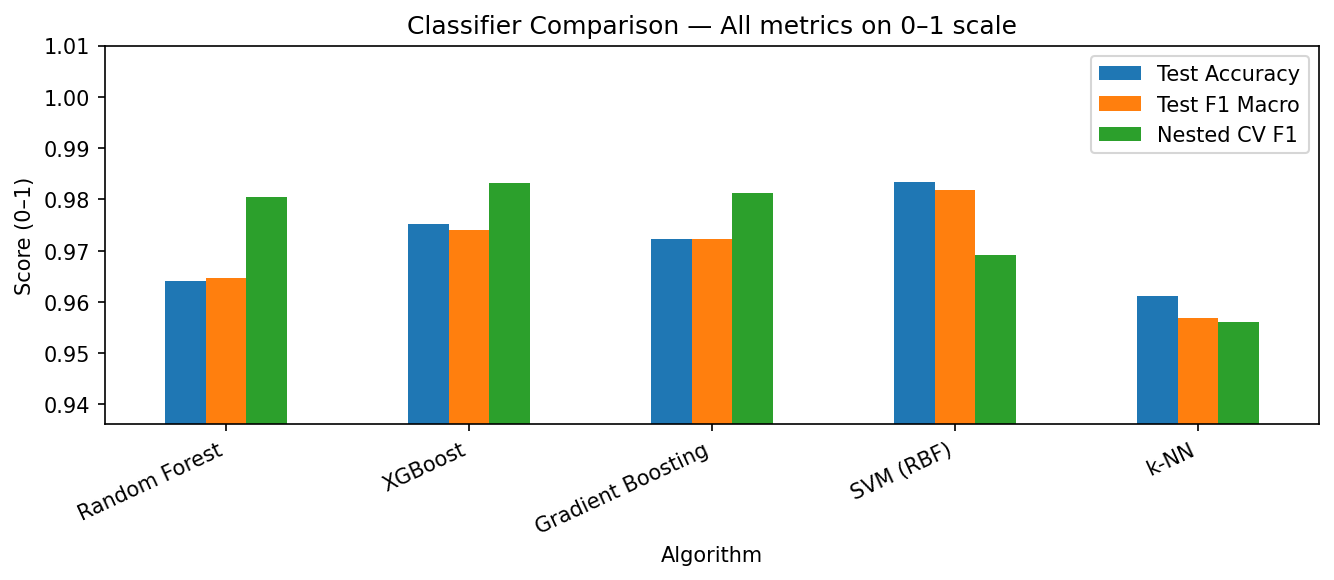
\includegraphics[width=\columnwidth]{fig5_accuracy_f1_comparison.png}
  \caption{Overall accuracy vs.\ macro F1-score comparison for all five
           classifiers.}
  \label{fig:accuracy_f1}
\end{figure}

\subsection{Per-Class Analysis}

Table~\ref{tab:perclass} details per-class precision, recall, and F1 for the
production Random Forest model on the 361-sample held-out test set (20 sampling
locations not seen during training).

\begin{table}[htbp]
  \caption{Per-Class Results --- Random Forest (Production Model)}
  \label{tab:perclass}
  \centering
  \renewcommand{\arraystretch}{1.2}
  \begin{tabular}{lcccc}
    \toprule
    \textbf{Class} & \textbf{Precision} & \textbf{Recall} & \textbf{F1} & \textbf{Support} \\
    \midrule
    Diseased (\textit{proxy}) & 0.983 & 0.950 & 0.966 & 181 \\
    Healthy  (\textit{proxy}) & 1.000 & 0.988 & 0.994 &  86 \\
    Stressed (\textit{proxy}) & 0.901 & 0.968 & 0.933 &  94 \\
    \midrule
    Macro                     & 0.961 & 0.969 & 0.965 & 361 \\
    \bottomrule
  \end{tabular}
\end{table}

The Healthy proxy class achieves perfect precision (1.000) with 0.988 recall
across 86 test observations. The Diseased proxy class attains 0.983 precision
with 0.950 recall across 181 test observations, which represent the largest
partition in the location-grouped test set. The Stressed proxy class achieves
the lowest precision (0.901) while maintaining 0.968 recall. Because the proxy
labels are derived from the same spectral composite as the input features, per-class
performance should be interpreted as \textit{spectral proxy separability}
within this fitted model rather than verified crop pathology detection accuracy.
Normalised confusion matrices for all five classifiers are shown in
Fig.~\ref{fig:confusion}.

\begin{figure}[htbp]
  \centering
  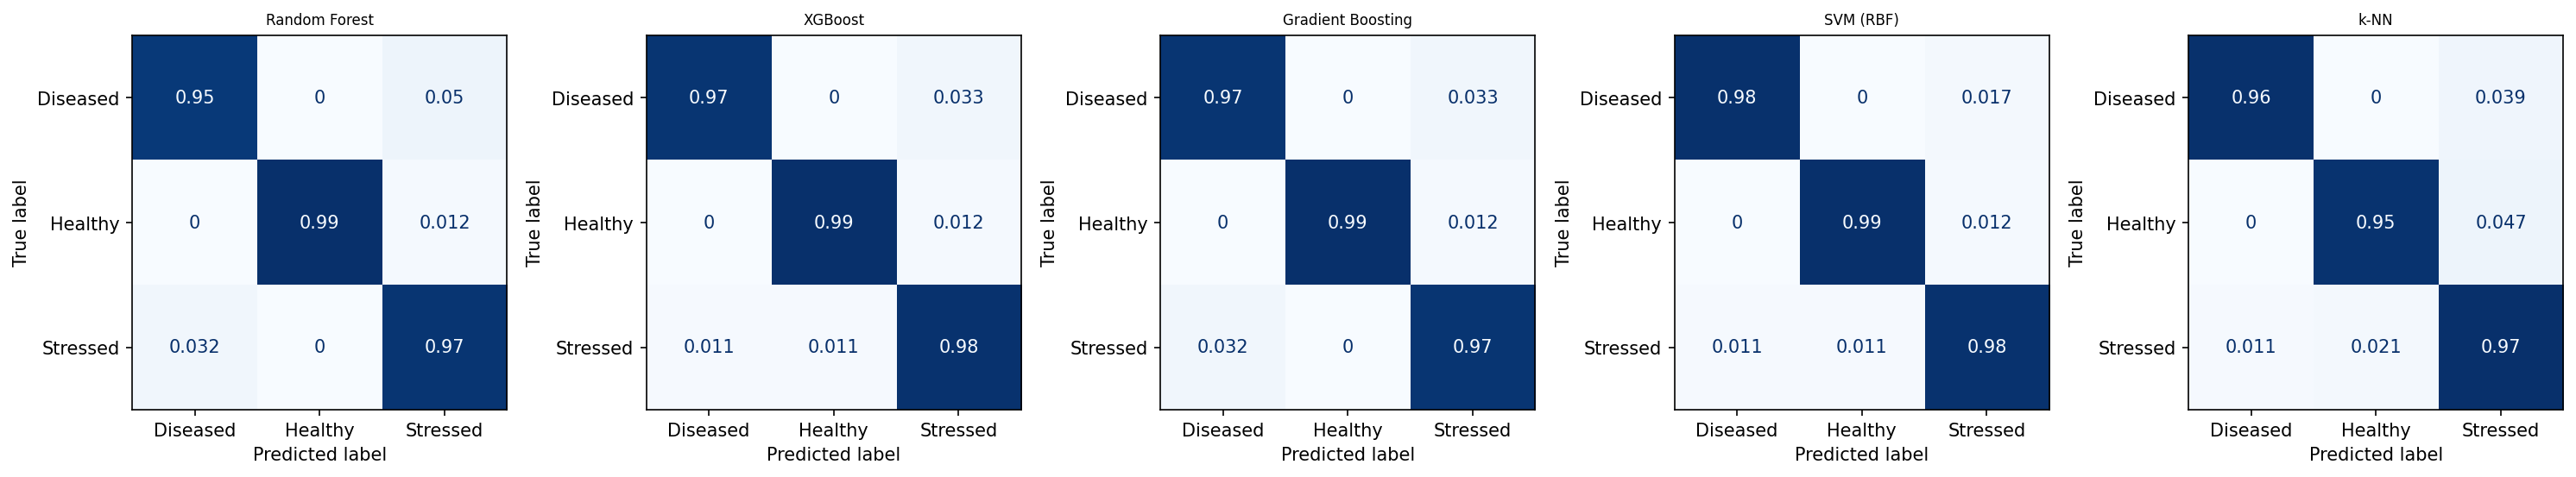
\includegraphics[width=\columnwidth]{fig3_confusion_matrices.png}
  \caption{Normalized confusion matrices for five classifiers on the
           held-out location-grouped test set (361 observations, 20 sampling
           locations). Cell values show normalized proportions; raw counts
           are not displayed.}
  \label{fig:confusion}
\end{figure}

\subsection{Feature Importance}

Table~\ref{tab:featimp} ranks the nine spectral features by importance for the
three tree-based models. Fig.~\ref{fig:featimp} provides a grouped bar chart.

\begin{table}[htbp]
  \caption{Native Feature Importance — Tree Models (impurity-based, sorted by RF).
           Caution: NDVI, NDRE, and EVI also appear in the label-generation rule,
           which inflates their apparent importance. Values are not directly
           comparable across algorithm families.}
  \label{tab:featimp}
  \centering
  \renewcommand{\arraystretch}{1.2}
  \begin{tabular}{clccc}
    \toprule
    \textbf{Rank} & \textbf{Feature} & \textbf{RF} & \textbf{XGBoost} & \textbf{GB} \\
    \midrule
    1 & NDVI      & 0.307 & 0.183 & 0.306 \\
    2 & LAI       & 0.249 & 0.646 & 0.371 \\
    3 & NDRE      & 0.236 & 0.134 & 0.302 \\
    4 & EVI       & 0.112 & 0.014 & 0.019 \\
    5 & NDVI\_max  & 0.042 & 0.002 & 0.000 \\
    6 & NDWI      & 0.040 & 0.005 & 0.001 \\
    7 & BSI       & 0.006 & 0.008 & 0.000 \\
    8 & NDVI\_min  & 0.005 & 0.005 & 0.001 \\
    9 & NDVI\_std  & 0.004 & 0.005 & 0.000 \\
    \bottomrule
  \end{tabular}
\end{table}

\begin{figure}[htbp]
  \centering
  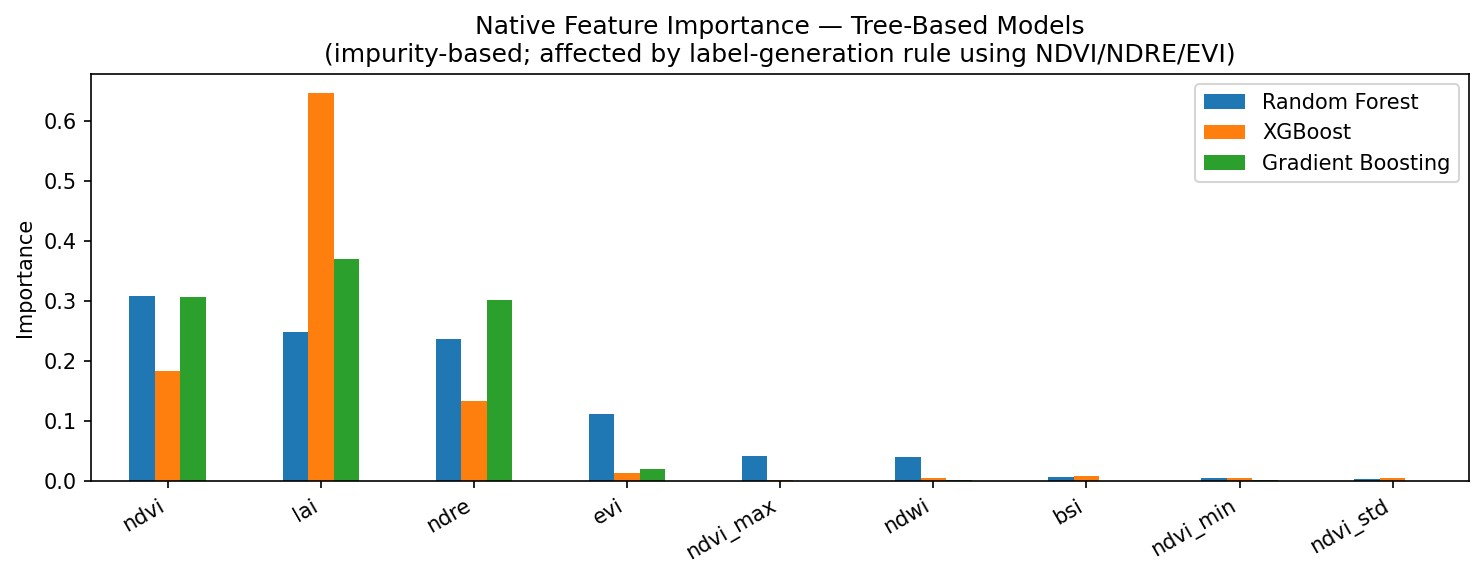
\includegraphics[width=\columnwidth]{fig4_feature_importance.png}
  \caption{Feature importances for Random Forest, XGBoost, and Gradient
           Boosting, sorted by Random Forest importance (descending).}
  \label{fig:featimp}
\end{figure}

NDVI, LAI, and NDRE are the three most informative features across all tree
models. For Random Forest, NDVI (0.307), LAI (0.249), and NDRE (0.236) together
account for 79\% of importance; EVI contributes 0.112 and the remaining five
features are near-zero. For XGBoost, LAI dominates strongly (0.646), with NDVI
(0.183) and NDRE (0.134) distant second and third. Gradient Boosting shows a
similar three-feature concentration: LAI (0.371), NDVI (0.306), NDRE (0.302).
NDWI, BSI, and all three temporal NDVI statistics (ndvi\_min, ndvi\_max,
ndvi\_std) are collectively below 0.05 in RF importance, suggesting limited
marginal discriminative power once the core spectral indices are included.

\textbf{Caution on circularity:} NDVI, NDRE, and EVI are the three indices that
define the crop\_stress\_label via a weighted composite.
Their high importance partly reflects the deterministic labelling rule rather than
independent biological variation; the reported ranking therefore measures
\emph{spectral proxy separability}, not confirmed agronomic importance.
LAI is a linear rescaling of EVI (LAI = 3.618$\cdot$EVI $-$ 0.118), so its
apparent dominance in boosted models is likely an artefact of that
transformation. The per-class F1 heatmap across all models is shown in
Fig.~\ref{fig:heatmap}.

\begin{figure}[htbp]
  \centering
  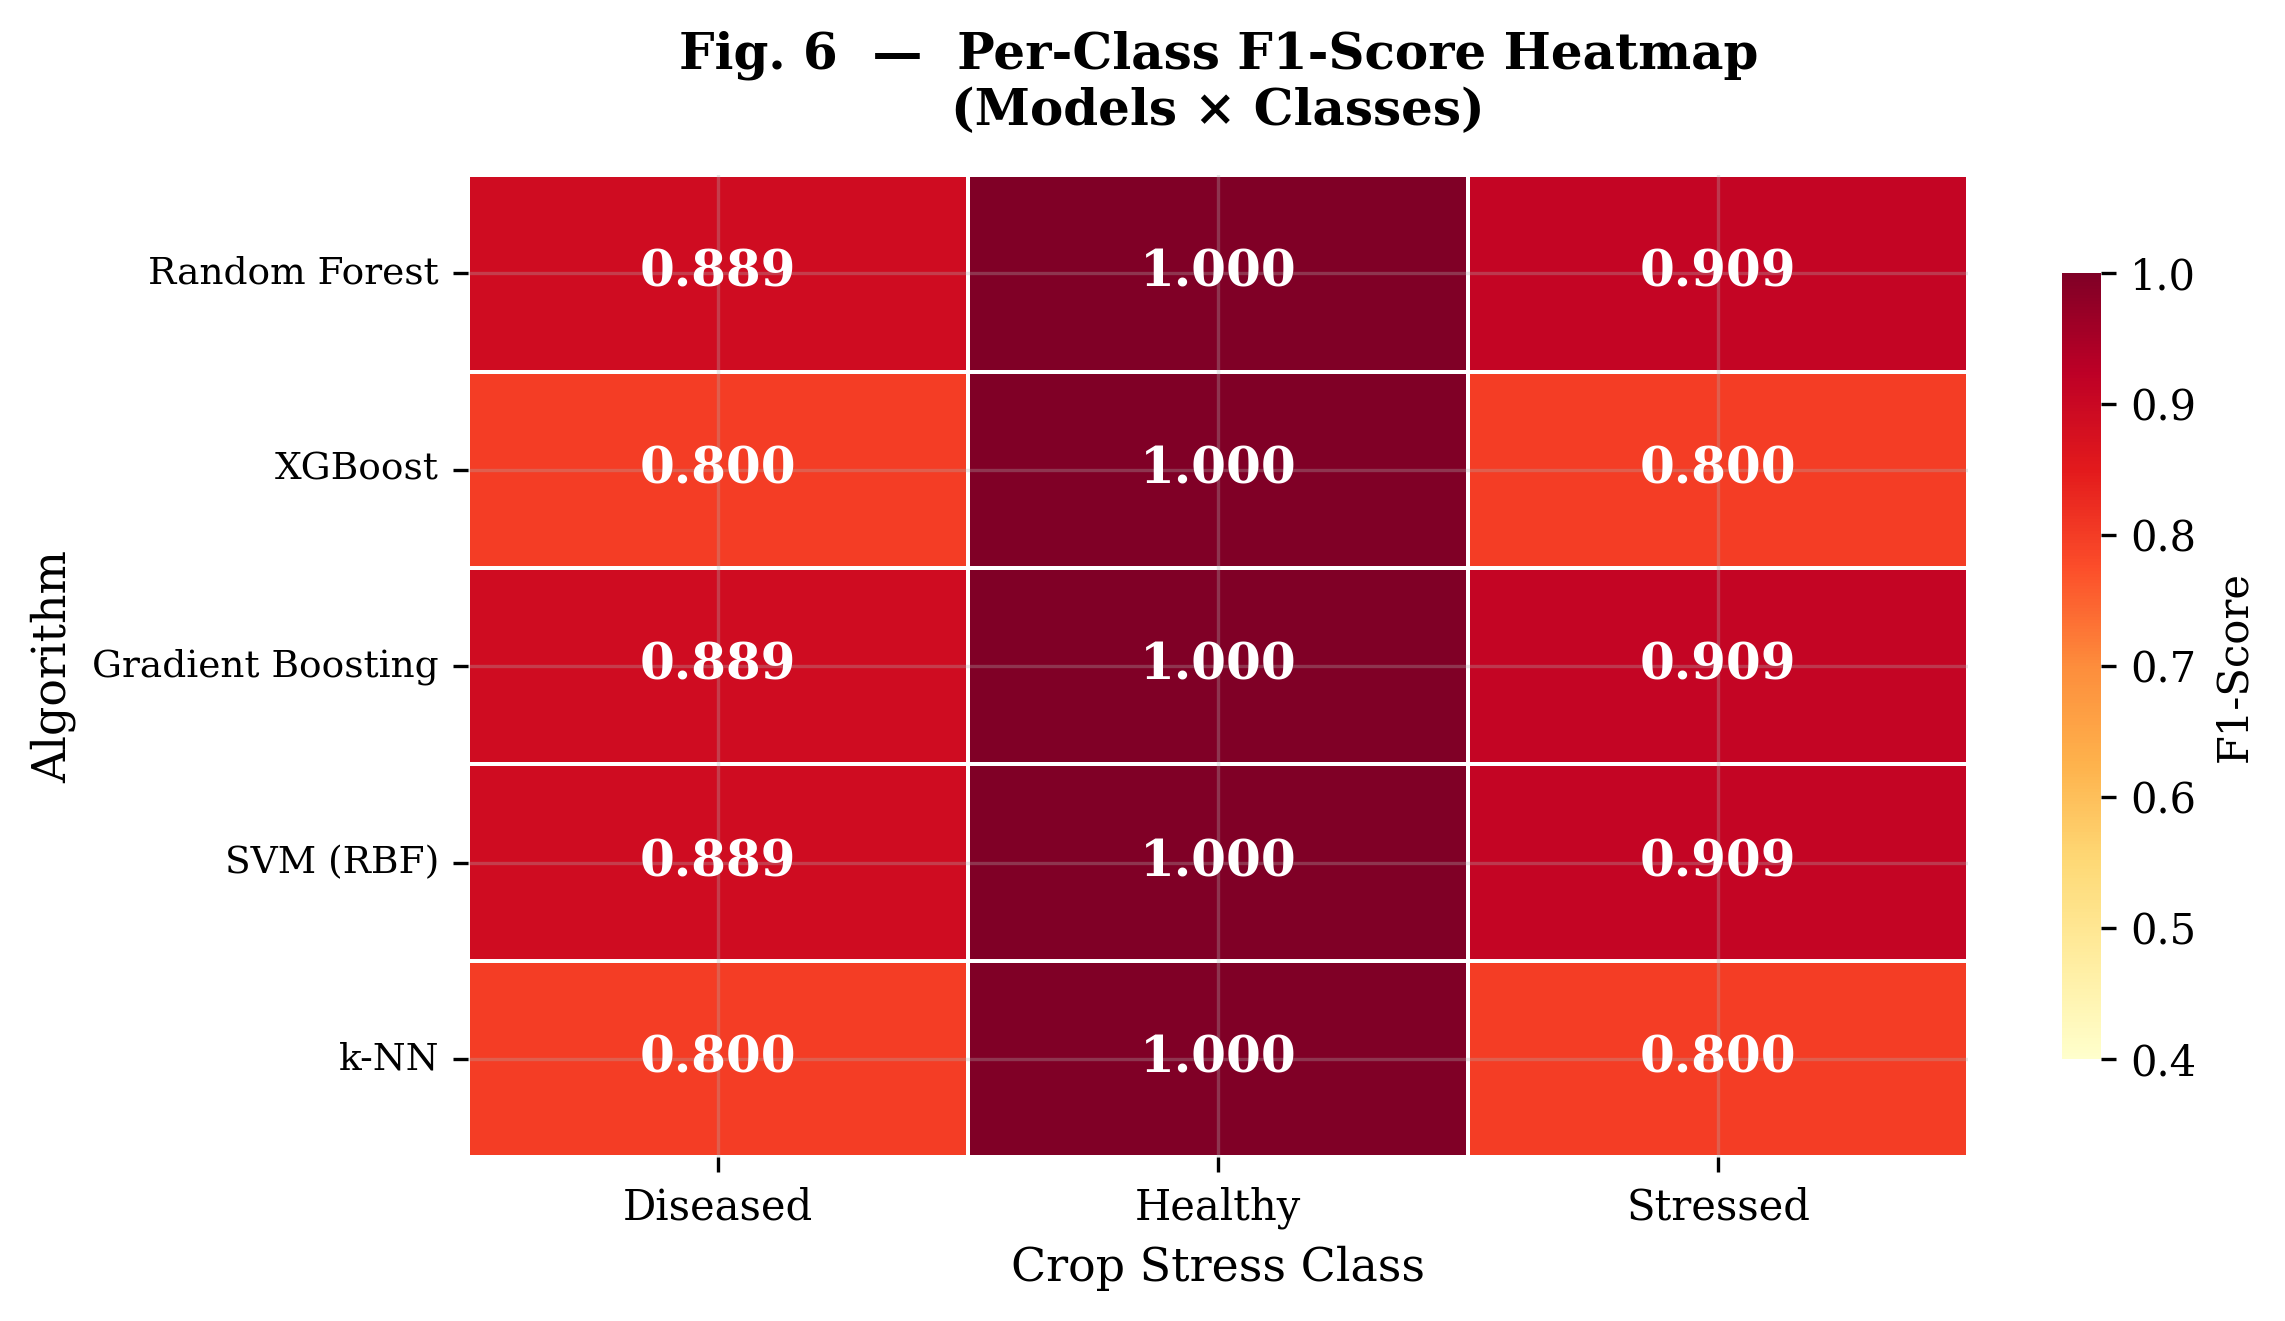
\includegraphics[width=\columnwidth]{fig6_perclass_f1_heatmap.png}
  \caption{Per-class F1-score heatmap across all five classifiers.}
  \label{fig:heatmap}
\end{figure}

\subsection{Discussion}

The results demonstrate that nine Sentinel-2 spectral features — six derived
indices and three temporal NDVI statistics — provide sufficient discriminative
signal for spectral proxy crop-condition classification across Pakistan's diverse
agronomic zones. Macro F1-score was selected as the primary optimisation
criterion to treat all three classes equally across their near-balanced support
(596 Healthy, 595 Stressed, 595 Diseased). The location-grouped nested
cross-validated macro F1 reached 0.9831 $\pm$ 0.0063 (XGBoost), 0.9813 $\pm$
0.005 (Gradient Boosting), and 0.9804 $\pm$ 0.0066 (Random Forest) on the
outer CV folds, with the held-out location-grouped test set yielding
0.9740 (XGBoost) and 0.9819 (SVM RBF).

\textit{Comparison with prior work requires a critical caveat}: Htitiou
\textit{et al.}~\cite{htitiou2020} reported 88\% overall accuracy using Random
Forest for crop-type mapping with ground-truth field surveys, and Maleki
\textit{et al.}~\cite{maleki2024} achieved F1 scores of 89.9--93.5\% for crop
mapping using multi-sensor fusion and in-situ reference data. These works used
independently verified class labels. By contrast, AgroSense labels are
\textit{spectrally derived} from the same NDVI, NDRE, and EVI values used as
features; the comparison is therefore not directly commensurate. Our high
F1 values partially reflect spectral proxy separability rather than independent
agronomic validation. Future work with GPS-surveyed, pathology-confirmed field
samples is needed for a fair cross-study comparison.

A key methodological contribution is the use of \textit{location-grouped}
train/test splitting: the dataset contains multiple seasonal observations per
sampling location, and a naive random split would allow the same location to
appear in both training and test partitions, inflating accuracy estimates.
By applying \texttt{GroupShuffleSplit} on location identifiers, the held-out
test set contains only sampling locations unseen during training, providing a
more conservative and realistic estimate of generalisation to new locations.
Similarly, nested cross-validation (5-fold outer / 3-fold inner
\texttt{StratifiedGroupKFold}) was used to avoid overfitting hyperparameter
selection to the validation split.

Reported metrics should be interpreted as spectral proxy classification
performance. Class labels are derived from the same vegetation indices used as
features; ground-truth field validation remains an important direction for future
work to establish independently verified crop-condition detection accuracy.

% ─────────────────────────────────────────────────────────────────────────────
\section{API Design}

The backend exposes a RESTful API with JWT bearer authentication. The API
follows resource-oriented design principles: each endpoint operates on a single
identifiable resource (farm, field, or analysis result) and is stateless across
requests, enabling independent horizontal scaling of the inference tier.
Table~\ref{tab:api} summarises the primary endpoints.

\begin{table*}[t]
  \caption{Summary of Primary API Endpoints}
  \label{tab:api}
  \centering
  \footnotesize
  \renewcommand{\arraystretch}{1.15}
  \begin{tabular}{p{6.2cm} p{2.4cm} p{7.8cm}}
    \toprule
    \textbf{Endpoint} & \textbf{Method} & \textbf{Purpose} \\
    \midrule
    \texttt{/auth/login}                        & POST            & Authenticate user; issue JWT access token \\
    \texttt{/auth/register}                     & POST            & Create new user account \\
    \texttt{/farms}                             & GET / POST      & List farms or create a new farm \\
    \texttt{/fields}                            & GET / POST / DELETE & Field CRUD with PostGIS boundary polygon \\
    \texttt{/imagery/\{field\_id\}}              & POST            & Trigger GEE satellite fetch and index computation \\
    \texttt{/ml/full-analysis/\{field\_id\}}     & GET             & Run all five ML models and return combined report \\
    \texttt{/ml/crop-stress/\{field\_id\}}       & GET             & Crop stress classification (Healthy / Stressed / Diseased) \\
    \texttt{/ml/irrigation/\{field\_id\}}        & GET             & Irrigation recommendation (4-class output) \\
    \texttt{/ml/yield/\{field\_id\}}             & GET             & Yield prediction (t/ha) and harvest readiness \\
    \texttt{/ml/soil/\{field\_id\}}              & GET             & Soil health (pH, salinity dS/m, organic matter \%) \\
    \texttt{/ml/vra-zones/\{field\_id\}}         & GET             & Variable-rate application zone mapping \\
    \texttt{/ml/export-pdf/\{field\_id\}}        & GET             & Generate and stream ReportLab PDF report \\
    \texttt{/ml/send-alert/\{field\_id\}}        & POST            & Dispatch crop health alert via Gmail SMTP \\
    \texttt{/weather/smart-farming/\{field\_id\}} & GET            & 7-day forecast, alert rules, and planting date scorer \\
    \bottomrule
  \end{tabular}
\end{table*}

% ─────────────────────────────────────────────────────────────────────────────
\section{Deployment}

The backend is containerised via Docker and deployed to Google Cloud Run
(us-central1), providing auto-scaling to zero for cost efficiency, a stable
HTTPS endpoint, and eliminating infrastructure management requirements. The PostgreSQL database
is hosted on a managed instance with the PostGIS~3~\cite{postgis} extension.
All third-party integrations (GEE, Open-Meteo, Gmail SMTP) are handled
server-side; the mobile client holds only a short-lived, revocable JWT token
with no embedded API keys.

% ─────────────────────────────────────────────────────────────────────────────
\section{Data and Code Availability}

The dataset (1,786 Sentinel-2 observations), training and evaluation scripts,
GEE data collection pipeline, Jupyter notebook, and a pre-trained Random Forest
production model are publicly available at:

\begin{center}
\url{https://github.com/ALI-SHAHMEER/agrosense-pakistan-crop-stress}
\end{center}

The repository includes a data dictionary, full methodology documentation, and
pinned dependency versions to support exact replication of the reported results.

% ─────────────────────────────────────────────────────────────────────────────
\section{Conclusion}

AgroSense demonstrates that satellite remote sensing, machine learning, and
real-time weather intelligence can be integrated into an accessible mobile
platform calibrated to the agronomic and linguistic context of Pakistan's
smallholder farming sector. Three findings emerge from this work. First, nine
Sentinel-2 spectral features (six derived indices and three temporal NDVI
statistics) provide sufficient discriminative signal for spectral proxy
crop-condition classification across all four provinces of Pakistan, with
SVM~(RBF) achieving the highest location-grouped held-out test accuracy
(98.34\%) and XGBoost achieving the best nested cross-validated macro F1
(0.983~$\pm$~0.006) — both under location-grouped evaluation. Reported
performance measures spectral proxy separability; class labels are derived
from the same spectral indices used as features, and independent field
validation is future work.
Second, location-grouped train/test separation (\texttt{GroupShuffleSplit} on
location identifiers) is essential for honest accuracy estimation when datasets
contain multiple seasonal observations per sampling location; naive random
splits inflate reported accuracy by allowing the same location to appear in
both partitions.
Third, a single stateless REST API deployed on Google Cloud
Run~\cite{googlecloudrun,fastapi} can serve both a Flutter mobile
application~\cite{flutter} and a PyQt6 desktop application, enabling
simultaneous support for field and office use cases without code duplication.

Future work will focus on ground-truth field validation of the spectrally
derived class labels, incorporation of multi-temporal deep learning
architectures, and formal user studies with smallholder farmers to evaluate
decision quality under real field conditions.

% ─────────────────────────────────────────────────────────────────────────────
\begin{thebibliography}{29}

\bibitem{pbs2024}
Pakistan Bureau of Statistics,
``Crop area and production statistics 2023--24,''
Islamabad, Pakistan, Tech.\ Rep., 2024. [Online]. Available: \url{https://mnfsr.gov.pk/SiteImage/Misc/files/ASP\%20for\%20Web\%202024.pdf}.

\bibitem{pesurvey2025}
Government of Pakistan, Finance Division,
``Pakistan Economic Survey 2024--25: Highlights,''
Economic Adviser's Wing, Islamabad, Pakistan, 2025. [Online]. Available: \url{https://finance.gov.pk/survey/chapter_25/Highlights.pdf}.

\bibitem{muzammil2020}
M.~Muzammil, A.~Zahid, and L.~Breuer,
``Water resources management strategies for irrigated agriculture in the
Indus Basin of Pakistan,''
\textit{Water}, vol.~12, no.~5, Art.\ no.~1429, 2020,
\href{https://doi.org/10.3390/w12051429}{doi: 10.3390/w12051429}.

\bibitem{drusch2012}
M.~Drusch \textit{et al.},
``Sentinel-2: ESA's optical high-resolution mission for GMES operational
services,''
\textit{Remote Sens.\ Environ.}, vol.~120, pp.~25--36, 2012,
\href{https://doi.org/10.1016/j.rse.2011.11.026}{doi: 10.1016/j.rse.2011.11.026}.

\bibitem{rouse1974}
J.~W. Rouse, R.~H. Haas, J.~A. Schell, and D.~W. Deering,
``Monitoring vegetation systems in the great plains with ERTS,''
in \textit{Proc.\ 3rd Earth Resources Technol.\ Satellite Symp.},
vol.~1, NASA SP-351, 1974, pp.~309--317. [Online]. Available: \url{https://ntrs.nasa.gov/api/citations/19740022614/downloads/19740022614.pdf}.

\bibitem{gitelson2002}
A.~A. Gitelson, Y.~J. Kaufman, R.~Stark, and D.~Rundquist,
``Novel algorithms for remote estimation of vegetation fraction,''
\textit{Remote Sens.\ Environ.}, vol.~80, no.~1, pp.~76--87, 2002,
\href{https://doi.org/10.1016/S0034-4257(01)00289-9}{doi: 10.1016/S0034-4257(01)00289-9}.

\bibitem{sishodia2020}
R.~P. Sishodia, R.~L. Ray, and S.~K. Singh,
``Applications of remote sensing in precision agriculture: A review,''
\textit{Remote Sens.}, vol.~12, no.~19, Art.\ no.~3136, 2020,
\href{https://doi.org/10.3390/rs12193136}{doi: 10.3390/rs12193136}.

\bibitem{gorelick2017}
N.~Gorelick, M.~Hancher, M.~Dixon, S.~Ilyushchenko, D.~Thau, and R.~Moore,
``Google Earth Engine: Planetary-scale geospatial analysis for everyone,''
\textit{Remote Sens.\ Environ.}, vol.~202, pp.~18--27, 2017,
\href{https://doi.org/10.1016/j.rse.2017.06.031}{doi: 10.1016/j.rse.2017.06.031}.

\bibitem{breiman2001}
L.~Breiman,
``Random forests,''
\textit{Mach.\ Learn.}, vol.~45, no.~1, pp.~5--32, 2001,
\href{https://doi.org/10.1023/A:1010933404324}{doi: 10.1023/A:1010933404324}.

\bibitem{chen2016xgboost}
T.~Chen and C.~Guestrin,
``XGBoost: A scalable tree boosting system,''
in \textit{Proc.\ 22nd ACM SIGKDD Int.\ Conf.\ Knowledge Discovery and
Data Mining}, New York, NY, USA: ACM, 2016, pp.~785--794,
\href{https://doi.org/10.1145/2939672.2939785}{doi: 10.1145/2939672.2939785}.

\bibitem{immitzer2016}
F.~Immitzer, F.~Vuolo, and C.~Atzberger,
``First experience with Sentinel-2 data for crop and tree species
classifications in Central Europe,''
\textit{Remote Sens.}, vol.~8, no.~3, Art.\ no.~166, 2016,
\href{https://doi.org/10.3390/rs8030166}{doi: 10.3390/rs8030166}.

\bibitem{tamiminia2020}
H.~Tamiminia \textit{et al.},
``Google Earth Engine for geo-big data applications: A meta-analysis and
systematic review,''
\textit{ISPRS J.\ Photogramm.\ Remote Sens.}, vol.~164, pp.~152--170, 2020,
\href{https://doi.org/10.1016/j.isprsjprs.2020.04.001}{doi: 10.1016/j.isprsjprs.2020.04.001}.

\bibitem{htitiou2020}
A.~Htitiou \textit{et al.},
``A comparative analysis of different phenological information retrieved from
Sentinel-2 time series images to improve crop classification: A machine
learning approach,''
\textit{Geocarto Int.}, vol.~37, no.~5, pp.~1426--1449, 2022,
\href{https://doi.org/10.1080/10106049.2020.1768593}{doi: 10.1080/10106049.2020.1768593}.

\bibitem{omia2023}
E.~Omia \textit{et al.},
``Remote sensing in field crop monitoring: A comprehensive review of sensor
systems, data analyses and recent advances,''
\textit{Remote Sens.}, vol.~15, no.~2, Art.\ no.~354, 2023,
\href{https://doi.org/10.3390/rs15020354}{doi: 10.3390/rs15020354}.

\bibitem{ojeilua2025}
C.~H. Ojeilua \textit{et al.},
``High-resolution stress detection in crops: Integrating satellite and drone
remote sensing for resilient agriculture,''
\textit{Afr.\ J.\ Agric.\ Sci.\ Food Res.}, vol.~19, no.~1,
pp.~447--467, 2025,
\href{https://doi.org/10.62154/ajasfr.2025.019.01037}{doi: 10.62154/ajasfr.2025.019.01037}.

\bibitem{karthikeyan2020}
L.~Karthikeyan, M.~Chawla, and A.~K. Mishra,
``A review of remote sensing applications in agriculture for food security:
Crop growth and production, irrigation, and crop losses,''
\textit{J.\ Hydrol.}, vol.~586, Art.\ no.~124905, 2020,
\href{https://doi.org/10.1016/j.jhydrol.2020.124905}{doi: 10.1016/j.jhydrol.2020.124905}.

\bibitem{maleki2024}
S.~Maleki \textit{et al.},
``Machine learning-based summer crops mapping using Sentinel-1 and
Sentinel-2 images,''
\textit{Remote Sens.}, vol.~16, no.~23, Art.\ no.~4548, 2024,
\href{https://doi.org/10.3390/rs16234548}{doi: 10.3390/rs16234548}.

\bibitem{wolfert2017}
S.~Wolfert, L.~Ge, C.~Verdouw, and M.-J. Bogaardt,
``Big data in smart farming --- a review,''
\textit{Agric.\ Syst.}, vol.~153, pp.~69--80, 2017,
\href{https://doi.org/10.1016/j.agsy.2017.01.023}{doi: 10.1016/j.agsy.2017.01.023}.

\bibitem{zippenfenig2023}
P.~Zippenfenig,
``Open-Meteo.com Weather API,''
\textit{Zenodo}, 2023,
\href{https://doi.org/10.5281/zenodo.7970649}{doi: 10.5281/zenodo.7970649}.

\bibitem{ashfaq2025}
M.~Ashfaq \textit{et al.},
``Predicting wheat yield using deep learning and multi-source environmental
data,''
\textit{Sci.\ Rep.}, vol.~15, Art.\ no.~26446, 2025,
\href{https://doi.org/10.1038/s41598-025-11780-7}{doi: 10.1038/s41598-025-11780-7}.

\bibitem{jamil2025}
M.~Jamil \textit{et al.},
``Remote sensing of wheat crop health in Punjab, Pakistan: Utilizing
Sentinel data and vegetation indices,''
\textit{Sir Syed Univ.\ Res.\ J.\ Eng.\ Technol.}, vol.~15, no.~2,
pp.~65--74, 2025,
\href{https://doi.org/10.33317/ssurj.705}{doi: 10.33317/ssurj.705}.

\bibitem{fastapi}
S.~Ram\'irez,
``FastAPI,'' version 0.111, 2024. [Online].
Available: \url{https://github.com/fastapi/fastapi}.

\bibitem{flutter}
Google LLC,
``Flutter software development kit,'' version 3.44, 2024. [Online].
Available: \url{https://flutter.dev}.

\bibitem{postgis}
Refractions Research,
``PostGIS spatial database extension,'' version 3.4, 2023. [Online].
Available: \url{https://postgis.net}.

\bibitem{reportlab}
ReportLab Europe Ltd.,
``ReportLab PDF library,'' version 4.2.5, 2024. [Online].
Available: \url{https://www.reportlab.com}.

\bibitem{clevers2013}
J.~G.~P.~W. Clevers and A.~A. Gitelson,
``Remote estimation of crop and grass chlorophyll and nitrogen content
using red-edge bands on Sentinel-2 and -3,''
\textit{Int.\ J.\ Appl.\ Earth Obs.\ Geoinf.}, vol.~23, pp.~344--351,
2013,
\href{https://doi.org/10.1016/j.jag.2012.10.008}{doi: 10.1016/j.jag.2012.10.008}.

\bibitem{xie2019}
Q.~Xie \textit{et al.},
``Retrieval of crop biophysical parameters from Sentinel-2 remote sensing
imagery,''
\textit{Int.\ J.\ Appl.\ Earth Obs.\ Geoinf.}, vol.~80, pp.~187--195,
2019,
\href{https://doi.org/10.1016/j.jag.2019.04.019}{doi: 10.1016/j.jag.2019.04.019}.

\bibitem{boiarskii2019}
B.~Boiarskii and H.~Hasegawa,
``Comparison of NDVI and NDRE indices to detect differences in vegetation
and chlorophyll content,''
\textit{J.\ Mech.\ Cont.\ Math.\ Sci.}, Special Issue, no.~4,
pp.~20--29, Nov.\ 2019,
\href{https://doi.org/10.26782/jmcms.spl.4/2019.11.00003}{doi: 10.26782/jmcms.spl.4/2019.11.00003}.

\bibitem{sklearn}
F.~Pedregosa \textit{et al.},
``Scikit-learn: Machine learning in Python,''
\textit{J.\ Mach.\ Learn.\ Res.}, vol.~12, pp.~2825--2830, Nov.\ 2011. [Online]. Available: \url{https://www.jmlr.org/papers/volume12/pedregosa11a/pedregosa11a.pdf}.

\bibitem{googlecloudrun}
Google LLC,
``Cloud Run — Fully managed serverless platform,'' 2024. [Online].
Available: \url{https://cloud.google.com/run}.

\end{thebibliography}

\end{document}
